%%% 雑誌会用 雛型ファイル 2015.7 %%%

%% コンパイルは (2回しましょう。)
% uplatex texファイル

%% pdfファイルにするには
% dvipdfmx -f uptex-ipaex.map dviファイル -o 出力ファイル名

% 認識の雑誌クラスを指定
\documentclass{zasshi-prml3}

% 必要なパッケージがあったら追加して
\usepackage{ascmac}%必須
\usepackage[dvipdfmx]{graphicx}
\usepackage[uplatex]{otf}
\usepackage{amsmath}
\usepackage{amssymb}
\usepackage{marvosym}
\usepackage{pifont}
\usepackage{tabularx}
\usepackage{url}

\DeclareMathOperator*{\argmin}{arg\,min}
\DeclareMathOperator*{\argmax}{arg\,max}
\usepackage{bm}
\usepackage{amsthm}
\theoremstyle{definition}
\newtheorem{theorem}{定理}
\newtheorem*{theorem*}{定理}
\newtheorem{definition}[theorem]{定義}
\newtheorem*{definition*}{定義}
%bibtexを使う場合、prml.bstを参照する
\bibliographystyle{prml}

% 雑誌会資料用コマンド
%
% I. 論文紹介 R. 自身の研究紹介 Q. 複数の研究をまとめて紹介 
%
\zasshi{15}     %: 雑誌会の回数(必須 in IRQ)  
\nendo{2019}       %: 雑誌会の年度(必須 in IRQ)
\title{gBoost: a mathematical programming approach to graph classification and regression}  %: 表題(必須 in IRQ)
\date{2019年7月22日(月) 15時00分}      %: 日付(必須 in IRQ)
\place{10-21}     %: 発表場所(省略可。省略時は10-21)
\presenter{白川 稜} %: 発表者(自分)(必須 in IRQ)
\abstract{
	グラフマイニング手法は、グラフ分類問題の特徴として利用することができる頻出な部分グラフパターンを列挙する.
	しかしながら,頻出な部分グラフパターンは必ずしも学習に有用であるとは限らない.
	ここでは,逐次的に有用なパターンを収集する数理計画ブースティング手法(gBoost)を提案する.
	既存のブースティング手法であるAdaBoostと比較して,
	gBoostはより少ないイテレーションで予測ルールを構築することができる.
	ブースティング手法をグラフデータに適用するため,
	分枝限定法を用いたパターン探索アルゴリズムをDFSコード木に基づき設計する.
	構築された探索空間は計算時間を最小化するため,後のイテレーションで再利用される.
	出力ラベルは探索空間を枝刈りするための情報源として利用されるため,
	本手法では頻出部分構造マイニングによる単純な方法よりも効率的な学習が可能である.
	加えて,数理計画問題を設計することで,
	パターン探索アルゴリズムの修正なしに広い範囲の機械学習の問題を解くことができる.
}  %: 概要(必須 in IRQ)
\journal{Machine Learning}   %: 雑誌名(必須 in IQ)
\vol{75}       %: 雑誌の volume(省略可)
\num{1}       %: 雑誌の number(省略可)
\year{2009}      %: 雑誌の発行年(必須 in IQ)
\page{69-89}      %: 論文の掲載ページ(必須 in IQ)
\author{Hiroto Saigo, Sebastian Nowozin, Tadashi Kadowaki, Taku Kudo, Koji Tsuda}    %: 論文の著者(必須 in IQ)

%  7つの質問に関する回答(全て必須)
% {}の中に記述する。

% Q.1 この論文(研究)の扱っているテーマは何か?
\ansfirst{部分グラフ支持子を特徴量としたグラフ分類問題.} %: 答えA.1

% Q.2 何故、この論文(研究)を取り上げたか? また、自分の研究との関連についても述べよ。
\anssecond{自身の研究のベースとなる手法であるため.} %: 答えA.2

% Q.3 これまでこのテーマに関する方法論の問題点は何か?
\ansthird{全部分グラフの総数はグラフサイズに対して指数関数的に増加するため,取り扱いが困難である.} %: 答えA.3

% Q.4 提案する方法論の独自性は何処にあり、どの点で有利と著者らは言ってい
% るか(と思うか)?また、どの点は不十分あるいは劣っているか?
\ansfourth{
	グラフ分類問題を線形計画問題として定式化し,列生成法のアイデアを元にブースティング手法を構築する.
	加えて特徴探索において,boundの取り方を与えbranch\&bound法を用いることで,
	従来では扱うことのできない数の特徴を考慮することが可能となる.
} %: 答えA.4

% Q.5 発表者の視点でこの論文を評価した場合、どこに利点があると思うか?
\ansfifth{従来では扱うことのできない数の特徴を考慮できる点とそれによる精度の向上.} %: 答えA.5

%TODO
% Q.6 発表者の視点でこの論文を評価した場合、どういう点が不十分であると思うか?
\anssixth{} %: 答えA.6

% Q.7 この論文(研究)を発展させる方向はどの辺にあるか?(できれば具体的なアイディアを述べよ)
\ansseventh{
	探索の効率化.branch\&bound法を用いた上でも探索空間が膨大であるため,
	厳密に探索を行うには相応のコストを要する.
	従って,MCTSやA*を用いた低コスト探索アルゴリズムの応用が有用であると考える.
} %: 答えA.7

% ※以上のコマンドは必ずプリアンブルで設定すること。
%   また、省略可というのは TeX compile に関してであって、
%   雑誌会資料においても省略可であるとは限らない。
% \Cite{str}      : 文献の参照(先頭を大文字に!)

% ※ #: 整数  str: 文字列

\begin{document}
% 以下本文(例)。普通のtex形式で。
% maketitleはしない。

\section{はじめに}
グラフは文書構造やRNA二次構造など様々な種類のものを表現することのできる重要なデータ構造である.
中でも一般的なのが化学構造の表現であり,活性・物性予測を機械で行う際に利用される.
予測に用いる特徴量として分子の性質に関するグラフ記述子がいくつか考案されてきたが,
タンパク質やRNA構造などの場合に関してのグラフ記述子は考案されていない.
よって,グラフデータと機械学習アルゴリズム間のインターフェースとなる特徴構築の方法が重要な問題となる.

この問題に対する一つの方法として,カーネル法が挙げられる.
カーネル法の基本的な考え方は、
グラフを部分構造(ウォークや木などの制約付き)の指示子の非常に高次元な空間として表現し,
2つの特徴ベクトル間の内積を再帰的アルゴリズムにより効率的に計算する.
カーネル法はすべての部分構造を考慮に入れるのだが,問題によっては考慮すべき特徴が少なくて良い場合や,
制約によって十分な特徴が作れない場合がある.
また,特徴が膨大かつ暗黙的であるため,予測ルールの解釈という点でも困難である.

他の方法として,頻出部分グラフマイニングを利用した方法がある.
この手法は,頻出部分グラフマイニングアルゴリズムを利用して列挙した頻出な部分グラフの指示子を特徴とし,
SVMなどの学習モデルにかける"2段階"の手法である.
しかし既存の研究によると,頻出度によって制約をかけることで
学習精度の低下を引き起こす可能性があることが知られている.
一方で頻出度制約を弱くすることは列挙する対象の増加につながり,
計算時間コスト及び計算メモリコストに関して実応用が困難という問題点が生じる.

これらの問題に対して,頻出部分グラフマイニングを
識別に有効な部分グラフのマイニングに置き換えることで改善を試みる手法が考案されている.
この手法は情報利得などの統計的な評価基準を利用して識別に有効な特徴を列挙し,
その指示子を特徴として学習モデルにかけるというものである.
しかしこの手法では,評価基準がその後の学習に大きく影響を与えるものであり,
統計的な評価基準が学習の特徴選択に有効であるという理論的な保証がない.

ここで本手法はLP-Boostと呼ばれる数理計画問題として定式化したブースティング手法と
部分グラフマイニングアルゴリズムを組み合わせることでグラフデータに対する学習モデルを構築する.
扱う部分グラフの総数は膨大であるが列生成法を用いて,段階的に特徴を追加していくことでこの問題を解決する.
本手法では目的関数の減少を観察することで最適解からのギャップを評価することができ,
終了条件を理論的に設定することができる.
また,特徴を繰り返し探索し一つずつ特徴集合に追加していくという反復アルゴリズムを設計するが,
探索アルゴリズムにおいて分枝限定法を利用することで計算コストの削減を図る.
探索空間はgSpanというアルゴリズムを元に構築されるDFSコード木を利用する.
各探索イテレーションでは利得関数による評価値を用いてDFSコード木より一つの特徴を探索する.
DFSコード木の構築には多くのコストを要するため木は保存して利用される.
愚直な方法では木を構築してから探索を順次行うのだが,
木を構築と探索を同時に行うことで余分なコストの削減を行う.

本手法はAdaBoostとパターン探索アルゴリズムを組み合わせた既存研究を元にしている.
しかし,AdaBoostは終了条件までの反復回数が多く時間コストがかかる.
実験ではグラフ分類のベンチマークであるQSARデータセットを用いてAdaBoostとの比較を行う.

\section{準備}
本研究ではラベル付き無向連結グラフを扱うため,はじめに定義を与える.
\begin{definition}(ラベル付き無向連結グラフ)
	ラベル付きグラフは4つのタプルで表現される,
	$G=(V, E, \mathcal{L}, l)$.
	ここで$V$はノード集合,$E \subseteq V \times V$はエッジ集合,$\mathcal{L}$はラベル集合,
	$l: V \cup E \rightarrow \mathcal{L}$はノードとエッジに割り当てるラベルのマッピングである.
	またラベル付き無向連結グラフは,上記のグラフのうち任意のノード間にパスが存在するものである.
\end{definition}

\section{グラフ分類問題}
\subsection{問題設定}
まずはじめに,グラフの二値分類問題を定義する.
この問題は,教師データとしてグラフ($G$)とそのクラスラベル($y \in \{+1, -1\}$)
のペアの集合$\{G_n, y_n\}^{\ell}_{n=1}$を与えられた際,
未知のグラフデータに対するクラスラベルを予測する予測器を学習する問題である.

\subsection{提案手法}
提案手法では特徴量として部分グラフ指示子を利用する.
教師データに少なくとも1回は出現する全ての部分グラフ集合を$\mathcal{T}$とすると,
グラフ$G_n$は$|\mathcal{T}|$次元のベクトル
$\bm{x}_n(x_{n,t} = \mathbb{I}(t \subseteq G_n), \forall t \in \mathcal{T})$として表現することができる.
$\mathbb{I}(\cdot)$は括弧内が真なら1,偽なら0を返す指示関数である.
特徴ベクトルの例を図\ref{feature_vec}に示す.
\begin{figure}[b]
	\centering
	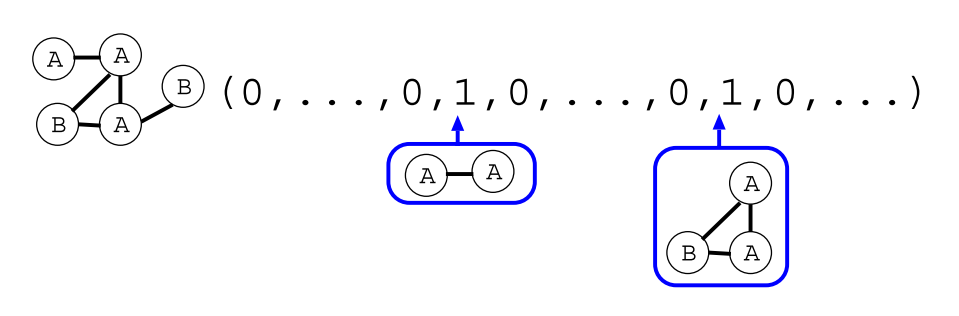
\includegraphics[width=100mm]{figure/feature_vec.png}
	\caption{特徴ベクトル(部分グラフ指示子)}
	\label{feature_vec}
\end{figure}

この二値の特徴表現に対して,仮説(hypothesis)と呼ばれる弱学習器(決定株)を以下で定義する.

\begin{equation*}
	h(\bm{x};t,\omega) = \omega (2x_t - 1).
\end{equation*}
$\omega \in \Omega = \{-1,1\}$はパラメータであり,
このパラメータにより部分グラフを含まないという情報も利用することができる.
この弱学習器を用いて,提案手法では以下の線形分類モデルを構築する.
\begin{align}
	\label{eq:linear}
	f(\bm{x}) = \sum_{(t,\omega) \in \mathcal{T}\times \Omega} \alpha_{t,\omega} h(\bm{x};t,\omega).
\end{align}
$\alpha_{t,\omega}$は各弱学習器の重みであり,$\sum_{(t,\omega) \in \mathcal{T}\times \Omega} \alpha_{t,\omega}=1,\alpha_{t,\omega} \geq 0$を満たす.

提案手法では,
LPBoostで定式化された以下の線形計画問題を主問題として解くことで,
式\eqref{eq:linear}の線形モデルの重み$\alpha_{t,\omega}$の値を導く.
\begin{align}
	&\min_{\bm{\alpha},\bm{\xi},\rho} -\rho + D \sum_{n=1}^{\ell} \xi_{i} \nonumber\\
				&\text{s.t.} \,\,\left\{
	\begin{aligned}
		&\sum_{(t,\omega) \in \mathcal{T} \times \Omega} y_{n} \alpha_{t,\omega} h(\bm{x_{n}};t,\omega) + \xi_{n} \geq \rho,
		\xi_{n} \geq 0,	n = 1, \dots , \ell,\nonumber \\
		&\sum_{(t,\omega) \in \mathcal{T} \times \Omega} \alpha_{t, \omega} = 1, \alpha_{t, \omega} \geq 0.
	\end{aligned}\right.
\end{align}
ここで,$\rho$はソフトマージン,$D=\frac{1}{\nu \ell}, \nu \in (0,1)$であり,$\ \nu\ $は誤分類に対するコスト制御のパラメータである.
一般に,変数$\bm{\alpha}$の数は部分グラフの総数であるため膨大であり,主問題を解くことは困難である.
したがって,主問題と等価な以下の双対問題を扱う.

\begin{align}
	\label{eq:dualprob}
	&\min_{\bm{\lambda},\gamma} \gamma \nonumber\\
	&\text{s.t.} \,\,\left\{
	\begin{aligned}
	& \sum_{n=1}^{\ell} \lambda_{n} y_{n} h(\bm{x}_{n};t,\omega) \leq \gamma,
	\forall(t,\omega) \in \mathcal{T} \times \Omega\\
	& \sum_{n=1}^{\ell} \lambda_{n} = 1, \,0 \leq \lambda_{n} \leq D, \,i = 1, \dots , \ell. 
\end{aligned}\right. \end{align}

双対問題は,主問題に比べ制約式の数は多くなるが列生成法を用いることで解を得ることが可能となる.
列生成法は,制約なしの状態から始め,現制約を最も違反する制約を追加し,
最適化問題を解くという過程を繰り返すことで解を得る手法である.
最も違反する制約を見つける問題は以下の最大化問題と等価である.
\begin{equation*}
	(t^{*}, \omega^{*}) = \argmax_{t \in \mathcal{T} , \omega \in \Omega} \sum_{n=1}^{\ell} \lambda_{n}^{(k)} y_{n} h(\bm{x_{n}} ; t, \omega).
\end{equation*}
$k$はイテレーション回数であり,$k=0,1,\ldots$.
便宜上最大化する右辺をgainと呼び以下の式で定義する.
\begin{align}
	\label{eq:gain}
	g(t, \omega) = \sum_{n=1}^{\ell} \lambda_{n}^{(k)} y_{n} h(\bm{x_{n}} ; t, \omega).
\end{align}
もし以下を満たすような$(t, \omega)\in \mathcal{T} \times \Omega$が存在しない,
つまり違反する制約が存在しない場合,その時点での解が双対問題の最適解となる.

\begin{equation*}
	 g(t, \omega) > \gamma^{(k)}.
\end{equation*}

経験的に終了付近の制約追加による重みの更新は僅かであるため,
緩和項$\ \epsilon \ $を用いて以下のように終了条件を緩和することで,計算を効率化する.
\begin{equation*}
	 g(t, \omega) > \gamma^{(k)} + \epsilon .
\end{equation*}
双対問題の終了条件緩和により得られる主問題の解を$V$,緩和なしでの最適解を$V^*$とすると,
$V \leq V^* + \epsilon$を満たす.\\

次に提案手法における特徴探索を考える.
特徴探索の方針は,探索空間中から最も大きなgainの特徴を探すことである.
特徴探索では重複無しに全部分グラフを列挙した探索空間であるDFSコード木(図\ref{dfscode_tree})を用いる.
\begin{figure}[t]
	\centering
	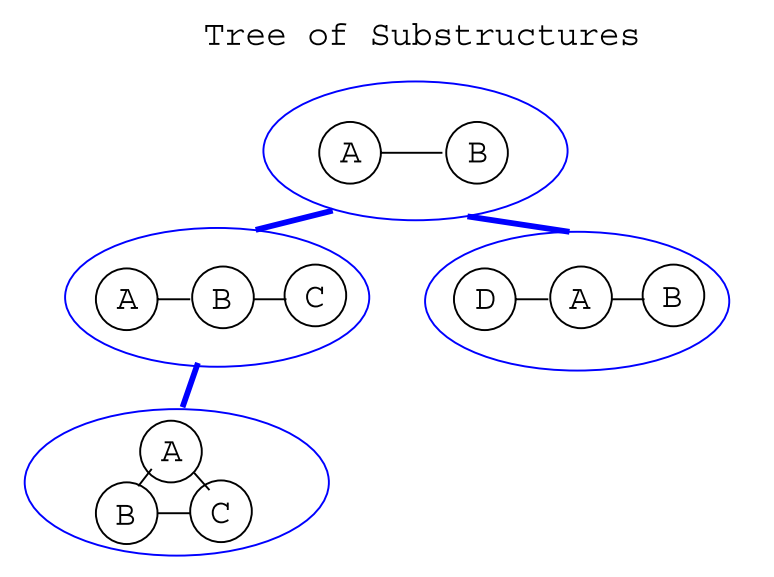
\includegraphics[width=70mm]{figure/dfscode_tree.png}
	\caption{DFSコード木}
	\label{dfscode_tree}
\end{figure}
DFSコード木は,教師データに含まれる全部分グラフをノードとして表現する探索空間であり,
子が親の拡大グラフとなるという特徴を持つ.
この探索木を深さ優先順にたどり,各ノードにおいてgainを計算することで,最適な(最大gainの)部分グラフを探索する.
一般に,部分グラフの総数は膨大となるため全てのノードを探索するためには相当なコストを要する.
しかし,子が親の拡大グラフとなる特徴を利用すると,
bound(子孫ノードでのgainの上限値)を計算することができるため,
安全な枝刈りを行うことが可能である.
boundの計算,枝刈り可能条件を以下に示す.

現探索部分グラフを$t$,その拡大グラフを$t'$とすると,
boundの値$b(t)$は以下の式で計算できる.
\begin{align}
	\label{eq:bound}
	b(t) = \max\{2 \sum_{\{n|y_{n}=+1, t \subseteq G_{n}\}} \lambda_{n}^{(k)} - \sum_{n=1}^{\ell} y_{n} \lambda_{n}^{(k)},	2 \sum_{\{n|y_{n}=-1, t \subseteq G_{n}\}} \lambda_{n}^{(k)} - \sum_{n=1}^{\ell} y_{n} \lambda_{n}^{(k)}\}.
\end{align}
枝刈り可能条件は,現探索までのgainの最大値を$g^{*}$とすると以下となる.
\begin{align}
	\label{eq:prune}
	g^{*} > b(t).
\end{align}
この枝刈りが有効に働くため,提案手法では探索空間に対して効率よくモデルを構築することができる.

提案手法のアルゴリズムを以下に示す.
\begin{figure}[h]
	\centering
	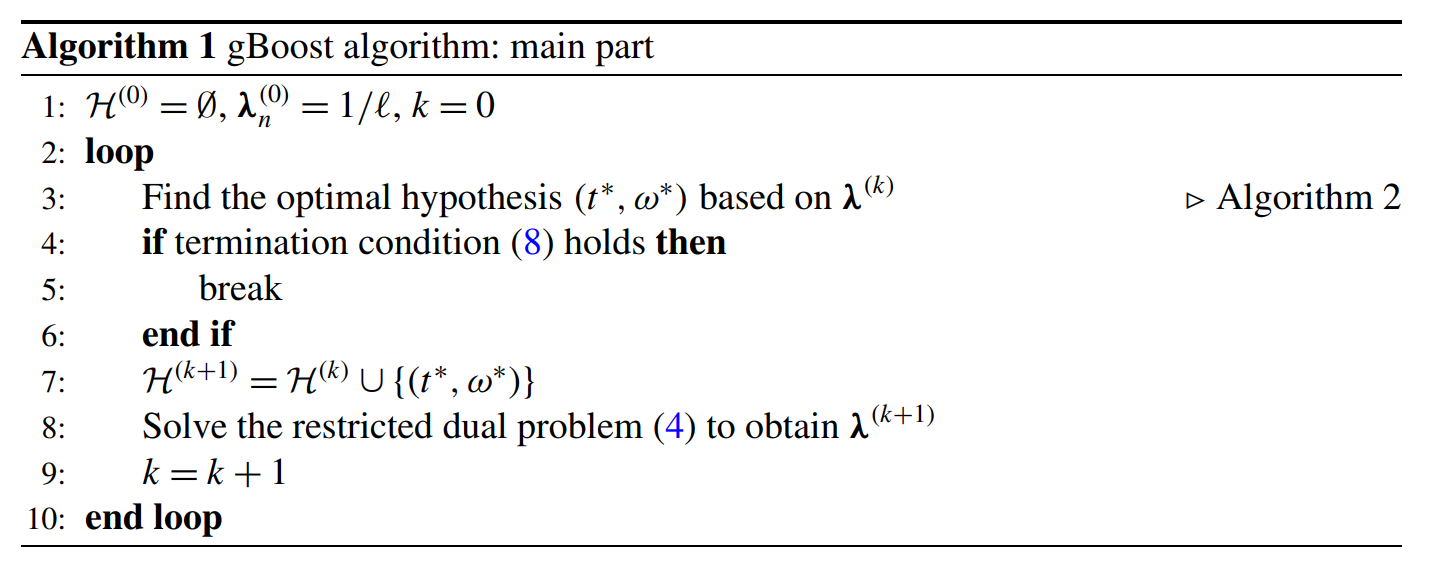
\includegraphics[width=140mm]{figure/algorithm1.png}
	\caption{LPBoost part}
	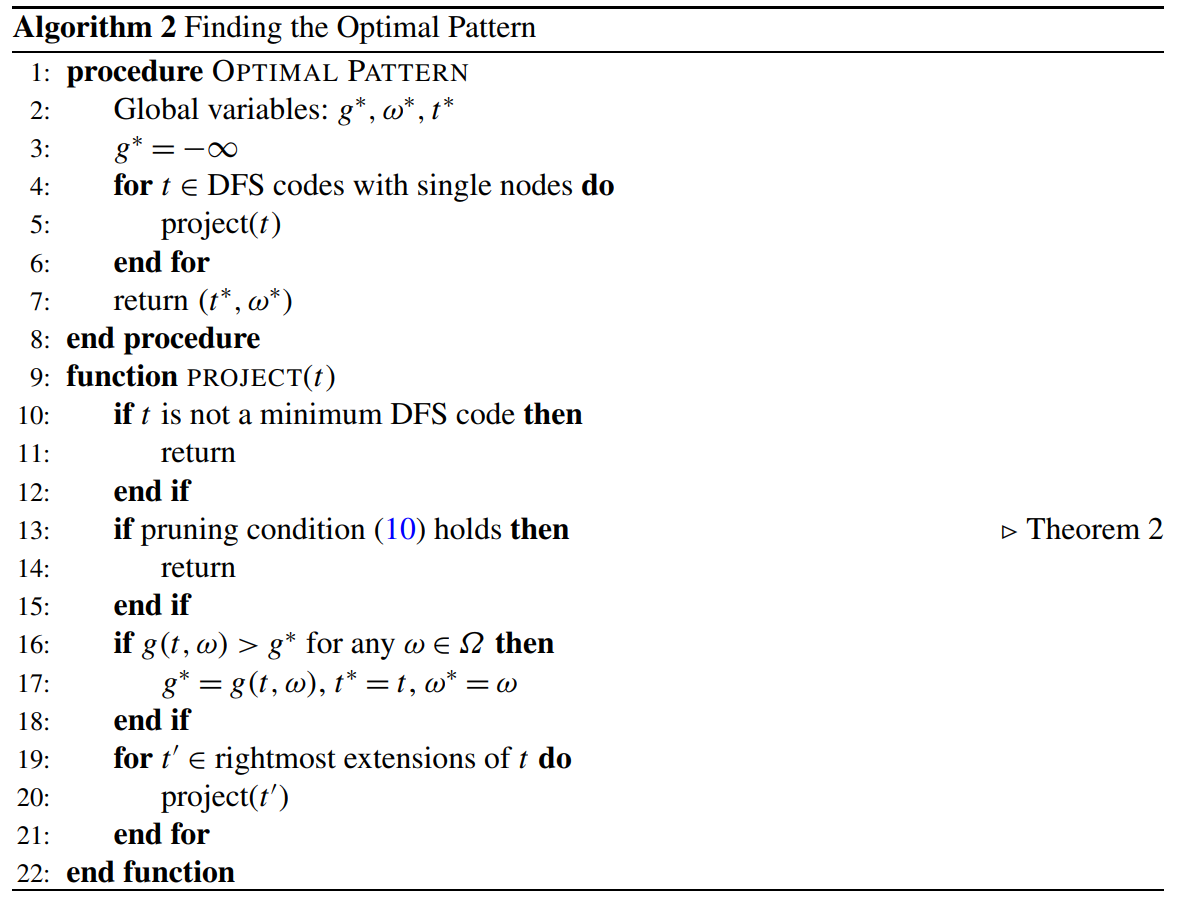
\includegraphics[width=140mm]{figure/algorithm2.png}
	\caption{feature search part}
\end{figure}

\section{実験}
\subsection{データセット}
グラフ分類問題のベンチマークであるQSARデータセットのうち,Mutag,CPDB,CAS,AIDSを用いて実験を行う.
書くデータの詳細は図\ref{datasets}に示す.
\begin{figure}[t]
	\centering
	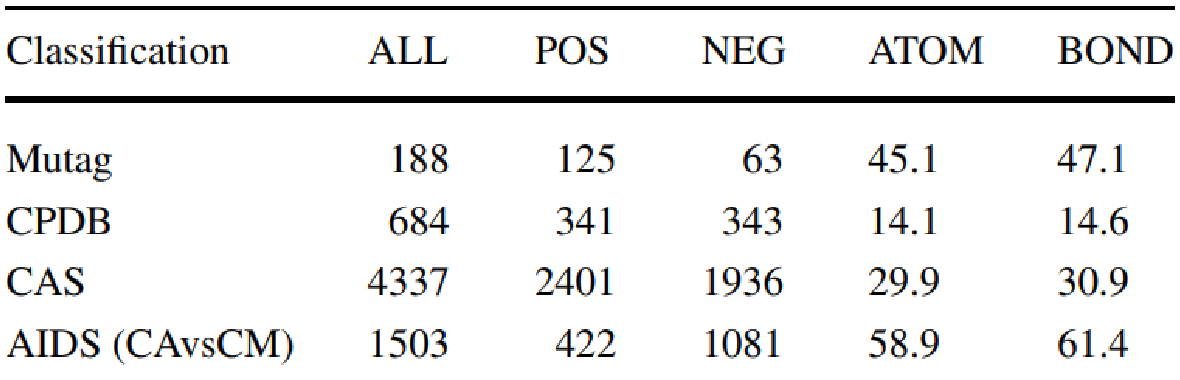
\includegraphics[width=110mm]{figure/datasets.png}
	\caption{データセット,ALL(全体グラフ数),POS(正例数),NEG(負例数),ATOM(原子数),BOND(結合数)}
	\label{datasets}
\end{figure}

\subsection{実験設定}

\subsection{結果}

\section{考察}

\section{今後の課題}

\begin{thebibliography}{9}
% 文献の書き方(別紙)参照
\bibitem{bib48}
T. Cazenave and N. Jouandeau, “A
parallel Monte-Carlo tree search
algorithm,” in
Proc. Comput. Games
, Beijing, China, 2008, pp. 72–80
\bibitem{bib80}
M. Enzenberger and M. Müller, “A
lock-free multithreaded Monte-
Carlo tree search algorithm,” in
Proc. Adv. Comput. Games
, Pamplona,
Spain, 2010, vol. 6048, pp. 14–20.
\end{thebibliography}

\end{document}
